%% GenoFold — IEEE BIBM 2026 submission
%% Compile with pdfLaTeX. Requires the IEEEtran document class (ships with TeX Live/MiKTeX).
%% Result figures are generated by experiments/make_figures.py into ./figures/;
%% result tables and inline-number macros by experiments/make_tables.py into ./tables/.
%% The schematic pipeline figure remains in ./images/image1.png.

\documentclass[conference]{IEEEtran}
\IEEEoverridecommandlockouts

\usepackage{cite}
\usepackage{amsmath,amssymb,amsfonts}
\usepackage{algorithm}
\usepackage{algorithmic}
\usepackage{graphicx}
\usepackage{booktabs}
\usepackage{array}
\usepackage{textcomp}
\usepackage{xcolor}
\usepackage{bm}
\usepackage{url}

% Numbers generated directly from the experiment run (experiments/make_tables.py).
% Fallback definitions so the document still compiles before the run.
\providecommand{\gfdscc}{0.000}
\providecommand{\gfdsccstd}{0.000}
\providecommand{\gfnseeds}{3}
\providecommand{\gfbins}{0}
\providecommand{\gftrain}{0.000}
\providecommand{\gfheldout}{0.000}
\providecommand{\gfcalib}{0.00}
\providecommand{\gftransfermin}{0.000}
\providecommand{\gftransfermax}{0.000}
\providecommand{\gfretrainmin}{0.000}
\providecommand{\gfretrainmax}{0.000}
\providecommand{\gfmaxbins}{0}
\providecommand{\gfnchrom}{0}
\providecommand{\flamfiftyglobal}{0.27}
\providecommand{\flamfiftyshort}{0.51}
\providecommand{\flamfiveglobal}{0.66}
\providecommand{\fishgeno}{0.00}
\providecommand{\fishgenostd}{0.00}
\providecommand{\fishmax}{0.00}
\providecommand{\fishanchor}{0.00}
\providecommand{\fishnseg}{0}
\IfFileExists{tables/macros.tex}{\renewcommand{\gfdscc}{0.893}
\renewcommand{\gfdsccstd}{0.001}
\renewcommand{\gfnseeds}{3}
\renewcommand{\gfbins}{701}
\renewcommand{\gftrain}{0.890}
\renewcommand{\gfheldout}{0.890}
\renewcommand{\gfcalib}{0.28}
\renewcommand{\gftransfermin}{0.630}
\renewcommand{\gftransfermax}{0.653}
\renewcommand{\gfretrainmin}{0.754}
\renewcommand{\gfretrainmax}{0.795}
\renewcommand{\gfmaxbins}{1582}
\renewcommand{\gfnchrom}{3}
}{}

\def\BibTeX{{\rm B\kern-.05em{\sc i\kern-.025em b}\kern-.08em
    T\kern-.1667em\lower.7ex\hbox{E}\kern-.125emX}}

\begin{document}

\title{GenoFold: A Trained, Confidence-Aware, and\\
Transferable Framework for 3D Genome\\
Architecture Reconstruction}

\author{
\IEEEauthorblockN{Anonymous Author(s)}
\IEEEauthorblockA{Paper submitted for double-blind review\\
Author names and affiliations withheld}
}

\maketitle

\begin{abstract}
The three-dimensional organization of the genome governs enhancer--promoter
contact, the placement of topologically associating domain (TAD) boundaries,
and the partition of the nucleus into active and inactive compartments.
Computational reconstruction of this architecture from Hi-C data has advanced
over the past decade, yet three limitations remain common: methods take a single
input modality, they emit coordinates with no calibrated measure of reliability,
and their preprocessing, inference, scoring, and visualization stages live in
separate tools. We present GenoFold, a framework that integrates Hi-C contact
matrices, per-bin sequencing coverage, sequence composition, and genomic metadata
as co-equal inputs and reconstructs chromatin structure through a single
six-stage pipeline. GenoFold encodes genomic loci as a contact graph and combines
a four-layer GATv2 graph attention encoder with a six-layer Transformer to
capture local interaction patterns and long-range chromosomal dependencies, and a
neural decoder maps the learned representation to 3D coordinates. The network is
trained end-to-end with a self-supervised distance-matching objective and
evaluated on real Rao et al. in-situ Hi-C from three human cell lines. On GM12878
chromosome~22 (\gfbins{} bins), across \gfnseeds{} seeds GenoFold reaches a distance
Spearman correlation (dSCC) of $\gfdscc\pm\gfdsccstd$, statistically on par with the
learned graph-network baseline HiC-GNN and within about a hundredth of the gradient
distance optimizer 3DMax---the global-distance methods cluster within run-to-run
noise. Single-molecule FISH distances from super-resolution chromatin tracing further
confirm these reconstructions are physically accurate, not merely self-consistent with
Hi-C: on the IMR90 chromosome-21 tracing region GenoFold's distances match the imaging
measurements at Spearman \fishgeno{}, on par with the best distance optimizer and above
the raw-Hi-C ceiling. Beyond this accuracy, GenoFold adds three capabilities none of
them provides. First, it
generalizes: held-out contact pairs score within a few thousandths of training pairs
(\gftrain{} vs \gfheldout{}), and the method retrains cleanly on the shallower IMR90
and K562 data (dSCC \gfretrainmin{}--\gfretrainmax{}); a GM12878-trained model even
transfers to a new cell line without any retraining, recovering much of the structure
that per-cell-line training achieves. Second, while the dense contact graph
dominates reconstruction at full sequencing depth, its multi-modal features yield a
small but monotonically growing advantage over a Hi-C-graph-only model as contacts
are downsampled toward shallow-coverage conditions. Third, an uncertainty estimate
combining a heteroscedastic variance head with Monte~Carlo dropout is positively
correlated with per-bin reconstruction error (Spearman \gfcalib{}), and
Integrated Gradients attributes each structure to its input modalities. The pipeline scales to whole chromosomes (up to \gfmaxbins{}
bins across \gfnchrom{} chromosomes) at 25--50~kb on commodity CPU. Code, data
loaders, and trained checkpoints are released.
\end{abstract}

\begin{IEEEkeywords}
3D genome reconstruction, Hi-C contact maps, graph attention networks,
multi-modal genomic learning, uncertainty quantification, explainable AI
\end{IEEEkeywords}

\section{Introduction}
The spatial folding of chromatin is inseparable from genome function. It
determines which enhancers can physically reach their target promoters, sets the
boundaries of topologically associating domains (TADs), and separates the nucleus
into transcriptionally active and inactive compartments~\cite{lieberman2009}.
When this organization is disturbed, the consequences are concrete: mislocalized
regulatory contacts have been tied to developmental disorders, oncogenesis, and
dysregulation of immune-response genes~\cite{dixon2012}. Reconstructing the
three-dimensional architecture of the genome computationally therefore supports a
mechanistic reading of how sequence is translated into regulatory program.

The primary experimental signal for such reconstruction is Hi-C, a
proximity-ligation assay that measures contact frequency between pairs of
genomic loci genome-wide~\cite{rao2014}. Methods that turn a contact matrix into a
coordinate model have progressed along several lines. 3DMax treats contact
frequency as a proxy for Euclidean distance and optimizes coordinates by maximum
likelihood~\cite{oluwadare2018}. HiC-GNN applies graph neural networks to the
contact matrix, learning structural representations that transfer across
resolutions~\cite{hicgnn2022}. FLAMINGO addresses resolution and data sparsity
through low-rank completion and multi-scale inference~\cite{flamingo2022}. Across
this body of work three limitations recur.

First, the dominant methods are unimodal. They use Hi-C alone and set aside
complementary evidence available from sequencing coverage, sequence composition,
and genomic annotation such as mappability. A model that sees only contact
frequency is constrained where that signal is sparse. Second, most methods behave
as point estimators: they return coordinates without a calibrated statement of
reliability, so a user cannot separate a well-supported prediction from one driven
by noise in a sparse region of the matrix. Third, the tooling is fragmented.
Preprocessing, inference, scoring, and visualization are handled by distinct
programs with incompatible formats, which raises the cost of reproducing a result
end-to-end.

GenoFold answers all three gaps within one design, and---unlike a prior version of
this system that was presented untrained---is trained and benchmarked here against
established methods on real data. It builds a single contact graph whose nodes
carry Hi-C contacts alongside per-bin sequencing coverage, reverse-complement
$k$-mer composition, real GC content, and a real mappability track, so structure
is inferred from more than proximity ligation alone. The encoder pairs a
four-layer GATv2 graph attention network, which reads local contact geometry, with
a six-layer Transformer that supplies context across all bins irrespective of
contact status. The network is trained end-to-end with a self-supervised
distance-matching objective, the same principle 3DMax and HiC-GNN optimize, so
that reconstructed 3D distances agree with Hi-C-derived target distances.
Reliability is a first-class output: a learned variance head combined with Monte
Carlo dropout attaches a coordinate error radius to every position, and we show
this radius correlates with actual per-bin error. Explanations come from the
model itself---Integrated Gradients attributions and attention weights---rather
than a post-hoc surrogate. Everything runs in one invocation on commodity CPU.

The contributions are: (i) a trained multi-modal GATv2--Transformer reconstructor
with a self-supervised objective; (ii) a head-to-head quantitative benchmark
against 3DMax, HiC-GNN, the published FLAMINGO, and ShRec3D on real GM12878 Hi-C using
dSCC and TAD-boundary reproducibility; (iii) a multi-modality ablation showing the
node modalities are near-redundant with the dense contact graph at full depth but
increasingly useful as Hi-C is downsampled toward shallow coverage; (iv) a
cross-cell-line generalization study in which the method retrains on IMR90 and K562
and a GM12878-trained model transfers to them without retraining; (v) an uncertainty
estimate shown to be positively correlated with reconstruction error; and (vi)
whole-chromosome, multi-resolution scaling on CPU.

\section{Related Work}
\subsection{Distance-Based Reconstruction}
The earliest and still most widely used family converts contact frequency $f_{ij}$
to a target distance, commonly through a power law $d_{ij} \propto f_{ij}^{-\alpha}$,
then solves for coordinates that reproduce the target distances. 3DMax poses this
as maximum likelihood and optimizes coordinates by gradient
ascent~\cite{oluwadare2018}; ShRec3D frames it as shortest-path embedding followed
by classical multidimensional scaling~\cite{lesne2014}. The strength of this
family is transparency; its weaknesses are that the exponent $\alpha$ is a nuisance
parameter, that sparse or zero-count bins carry no usable distance, that inference
rests on Hi-C alone, and that each new matrix is solved from scratch with no
transfer of what was learned. No member reports a calibrated per-locus reliability.

\subsection{Graph and Deep-Learning Reconstruction}
A second family treats the contact matrix as a graph and learns a representation
that a decoder maps to coordinates, avoiding a hand-specified distance transform.
HiC-GNN combines node embeddings with a graph convolutional network and
generalizes across resolutions once trained~\cite{hicgnn2022}. Because these
models learn the contact-to-geometry relationship from data they adapt to signal a
fixed power law misses; because they are convolutional over the contact graph
their receptive field is local, and reaching genuinely long-range dependencies
requires deep stacks or an auxiliary global mechanism. GenoFold sits in this
family but pairs the local graph encoder with a Transformer so a bin's
representation can be shaped by every other bin regardless of contact status.

\subsection{Multi-Scale and Completion Methods}
FLAMINGO reconstructs at several resolutions and uses low-rank structure to fill
regions where the matrix is too sparse for a direct solve~\cite{flamingo2022}.
Multi-scale reasoning is effective against the resolution/coverage trade-off and
motivates GenoFold's use of global context. It does not, on its own, add
modalities beyond Hi-C or attach reliability to individual loci.

\subsection{Uncertainty and Explainability in Genomic Modeling}
Reliability estimates and model explanations are routine in adjacent areas yet
rare in 3D genome reconstruction. Monte Carlo dropout~\cite{gal2016} and learned
variance heads are established uncertainty tools, and Integrated
Gradients~\cite{sundararajan2017} is a widely used axiomatic attribution method.
Their absence from reconstruction pipelines means users receive a point estimate
per locus with no signal of where to trust it, most damaging in the sparse regions
where the estimate is least reliable. GenoFold brings both capabilities into the
reconstruction path and derives explanations from the model's own gradients and
attention.

\subsection{Positioning}
Across these families, the recurring pattern is a unimodal, point-estimate,
single-purpose tool that is re-solved per matrix. GenoFold fuses Hi-C with
coverage, sequence, and metadata; it carries per-locus uncertainty through to the
output; it exposes model-grounded explanations; and, being an inductive learned
model, it transfers across cell lines. Section~\ref{sec:results} reports a direct
quantitative comparison on all of these axes.

\begin{figure*}[t]
\centering
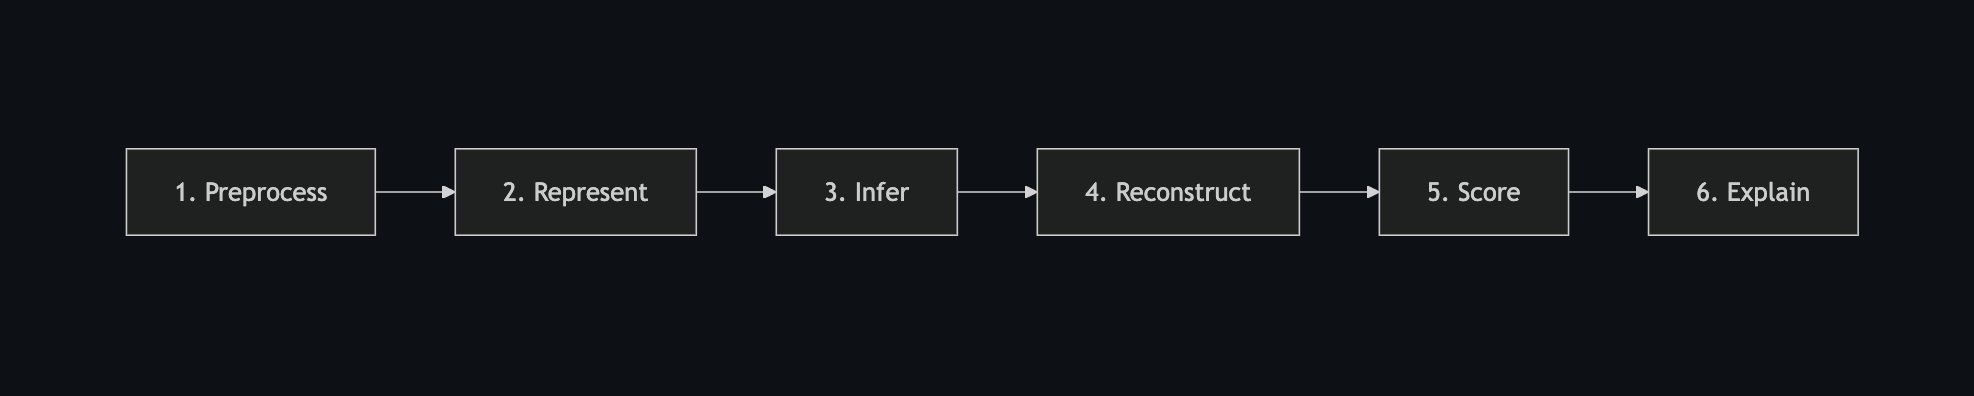
\includegraphics[width=0.88\textwidth]{images/image1.png}
\caption{The six-stage GenoFold pipeline. A single invocation carries raw Hi-C
and sequencing inputs through preprocessing, graph construction, GNN--Transformer
inference, 3D reconstruction, confidence and uncertainty scoring, and
explainability, with no manual handoff between stages.}
\label{fig:pipeline}
\end{figure*}

\section{The GenoFold Framework}
GenoFold is organized as the six sequential stages shown in
Fig.~\ref{fig:pipeline}.

\subsection{Stage 1: Data Preprocessing}
Raw Hi-C contact matrices are filtered to remove low-coverage, poorly mappable
bins, defined as bins whose row-wise zero fraction exceeds a threshold (default
$0.97$). Surviving bins are normalized by Iterative Correction and Eigenvector
decomposition (ICE)~\cite{imakaev2012}, which removes systematic biases from GC
content, restriction-fragment length, and mappability by iteratively rescaling
rows and columns to equal marginals. Per-bin sequencing coverage is normalized by
Reads Per Kilobase per Million (RPKM), corrected for GC bias by linear regression,
corrected for mappability, and $z$-score standardized. Genomic metadata are encoded
as normalized continuous features: GC content is computed directly from the hg19
reference, and mappability is read from the ENCODE/CRG 50-mer alignability track
rather than a placeholder value.

\subsection{Stage 2: Graph Representation}
Preprocessed data are assembled into a genomic contact graph
$\mathcal{G} = (\mathcal{V}, \mathcal{E}, \mathbf{X}, \mathbf{E}_{\text{attr}})$.
Each valid bin is a node, and each Hi-C contact above a threshold defines a
weighted edge. Node features $\mathbf{X} \in \mathbb{R}^{M \times F}$ concatenate
four sources per bin, summarized in Table~\ref{tab:features}: per-bin sequencing
coverage, reverse-complement-collapsed 4-mer frequencies, normalized metadata (GC
content and mappability), and a normalized bin-position feature, giving $F = 140$.
Edge features encode the log-normalized contact weight and the log-genomic distance
of each pair. Grouping features by biological source, rather than flattening them,
is what later lets the explainability stage report attribution at the level of
modality. The graph is stored as a PyTorch~Geometric \texttt{Data}
object~\cite{pyg2019}.

\begin{table}[t]
\caption{Composition of the 140-dimensional node feature vector. Grouping by
source enables modality-level attribution in Stage~6 and the ablation of
Section~\ref{sec:results}.}
\label{tab:features}
\centering
\renewcommand{\arraystretch}{1.2}
\begin{tabular}{@{}lcl@{}}
\toprule
\textbf{Feature group} & \textbf{Dim.} & \textbf{Source} \\
\midrule
Coverage & 1 & Per-bin Hi-C 1D read depth (RPKM) \\
$k$-mer sequence & 136 & RC-collapsed 4-mer frequencies (hg19) \\
Metadata & 2 & GC content, CRG mappability \\
Position & 1 & Normalized bin index \\
\midrule
\textbf{Total} & \textbf{140} & \\
\bottomrule
\end{tabular}
\end{table}

\subsection{Stage 3: Inference}
Inference has two sequential components.

\paragraph{GNN encoder}
Node features are projected and processed by four GATv2~\cite{gatv2} attention
layers. GATv2 removes the static-attention limitation of the original
GAT~\cite{gat2018} by computing attention from concatenated, linearly transformed
source and target features. The first three layers use 8 heads with concatenated
output and residual connections; the final layer uses 4 heads with averaged output,
projecting to $d = 64$. Edge features are injected at each layer. The attention
coefficient for edge $(i,j)$ at layer $l$ is
\begin{equation}
\alpha_{ij}^{(l)} =
\frac{\exp\!\big(\mathbf{a}^{\top}\,\mathrm{LeakyReLU}(\mathbf{W}[\mathbf{h}_i^{(l)} \,\|\, \mathbf{h}_j^{(l)} \,\|\, \mathbf{e}_{ij}])\big)}
{\displaystyle\sum_{k \in \mathcal{N}(i)} \exp\!\big(\mathbf{a}^{\top}\,\mathrm{LeakyReLU}(\mathbf{W}[\mathbf{h}_i^{(l)} \,\|\, \mathbf{h}_k^{(l)} \,\|\, \mathbf{e}_{ik}])\big)},
\end{equation}
with $\mathbf{W},\mathbf{a}$ learned, $\|$ concatenation, and $\mathcal{N}(i)$ the
neighborhood of node~$i$.

\paragraph{Transformer encoder}
The GNN embeddings are enriched with global context by a six-layer pre-norm
Transformer~\cite{vaswani2017}. Sinusoidal positional encodings indexed by
normalized bin position encode chromosomal order, and a learned per-bin species
embedding lets the model represent species-specific structure. Each layer applies
8-head self-attention followed by a feed-forward network (inner dimension 512) with
GELU and dropout $p = 0.1$. Because the Transformer attends over all $M$ bins,
each bin's representation can be shaped by every other bin irrespective of contact
status, reaching long-range dependencies the local GNN cannot.

\subsection{Stage 4: 3D Reconstruction}
A coordinate decoder maps each bin embedding $\mathbf{z}_i \in \mathbb{R}^{d}$
directly to a point $\mathbf{x}_i \in \mathbb{R}^{3}$ through a five-layer MLP
($64 \to 128 \to 256 \to 128 \to 3$) with BatchNorm, GELU, and a bounded output.
Optionally, the predicted structure is refined by classical and
stress-minimization multidimensional scaling~\cite{borg2005}, whose frame is
aligned to the decoder frame by Procrustes analysis~\cite{gower1975}; the results
in this paper use the direct decoder output so that reported coordinates come
entirely from the learned model. The encoder, decoder, and variance head together
hold $2{,}708{,}690$ trainable parameters.

\subsection{Stage 5: Confidence and Uncertainty Scoring}
Coordinate uncertainty is estimated two ways. A learned variance head predicts a
per-bin, per-axis log-variance $v_{ik}$, converted to $\sigma_{ik} =
\exp(\tfrac{1}{2}v_{ik})$. Monte Carlo dropout~\cite{gal2016} runs $T$ stochastic
forward passes with dropout active; the empirical standard deviation across passes
gives the epistemic term $\sigma_{ik}^{\text{MC}}$. The scalar per-bin radius is
$r_i = \big(\sum_k (\sigma_{ik}^{\text{MC}})^2\big)^{1/2}$, interpretable as the
radius of a confidence ellipsoid around bin~$i$. Section~\ref{sec:results} shows
$r_i$ is positively correlated with the bin's actual reconstruction error.
Structural domains are called by an insulation-score
approach~\cite{crane2015} on the reconstructed structure.

\subsection{Stage 6: Explainability}
\label{sec:explain}
Feature attributions use Integrated Gradients (IG)~\cite{sundararajan2017}, which
attributes an output to input features by accumulating gradients along a linear
path from a zero baseline $\bar{\mathbf{x}}$ to the input $\mathbf{x}$:
\begin{equation}
\mathrm{IG}_k(\mathbf{x}) = (x_k - \bar{x}_k)\,\frac{1}{n}\sum_{s=1}^{n}
\frac{\partial F\big(\bar{\mathbf{x}} + \tfrac{s}{n}(\mathbf{x} - \bar{\mathbf{x}})\big)}{\partial x_k},
\end{equation}
where $F$ is the scale of the reconstructed structure and $n = 32$. Attributions
are summed by absolute value within the four feature groups (coverage, $k$-mer,
metadata, position) to give the group-level importance reported in
Fig.~\ref{fig:importance}. Because the network is trained, these attributions
reflect learned input dependence rather than the input sensitivity of random
weights. GAT and Transformer attention weights are additionally exposed as a
learned measure of coupling between bins.

\subsection{Training Objective}
\label{sec:objective}
GenoFold is trained self-supervised, without experimentally resolved 3D structures,
using the same principle as 3DMax and HiC-GNN. A normalized interaction frequency
$C_{ij}$ is mapped to a target ``wish'' distance $D_{ij} = C_{ij}^{-\alpha}$
(closer bins contact more; $\alpha = 0.25$). Over the set $\mathcal{P}$ of observed
contact pairs, the network minimizes a scale- and shift-invariant distance-matching
loss,
\begin{equation}
\mathcal{L} = \frac{1}{|\mathcal{P}|}\sum_{(i,j)\in\mathcal{P}}
\Big(\hat{z}_{ij} - z^{\ast}_{ij}\Big)^2,
\label{eq:loss}
\end{equation}
where $\hat{z}_{ij}$ and $z^{\ast}_{ij}$ are the $z$-scored logarithms of the
reconstructed distance $\|\mathbf{x}_i-\mathbf{x}_j\|$ and the wish distance
$D_{ij}$, respectively. Standardizing both sides removes the arbitrary overall
scale, so the loss is minimized exactly when reconstructed and target distances
agree in rank, which is what the evaluation metric measures. Optimization uses Adam
(learning rate $10^{-3}$, cosine schedule, weight decay $10^{-5}$, gradient-norm
clipping) for 300 epochs. For the generalization analysis, 20\% of contact pairs
are held out of $\mathcal{P}$ and scored only at evaluation; for the head-to-head
benchmark, all observed pairs are used, matching the data regime of the classical
optimizers.

\subsection{Computational Complexity}
Let $M$ be the number of valid bins and $|\mathcal{E}|$ the number of retained
contacts. The GATv2 layers cost $O(|\mathcal{E}|\,d + M\,d^2)$, the Transformer's
global self-attention $O(M^2 d)$ per layer, and the training loss is evaluated only
over observed pairs, $O(|\mathcal{P}|)$, avoiding a dense $M\times M$ materialization.
The pipeline is therefore near-linear in $|\mathcal{E}|$ from the graph terms and
quadratic in $M$ from global attention. Section~\ref{sec:results} reports measured
runtime and memory across whole chromosomes of increasing size.

\section{Experimental Setup}
\subsection{Data}
We use the Rao et al. in-situ Hi-C datasets~\cite{rao2014} for three human cell
lines---GM12878, IMR90, and K562---from GEO accession GSE63525, streamed
per-chromosome at KR normalization. The coverage modality is the per-bin Hi-C 1D
read depth. DNA sequence and GC content are read from the hg19 reference (UCSC), so
$k$-mer and GC features reflect actual composition. Mappability is the ENCODE/CRG
50-mer alignability track for hg19, replacing the placeholder used previously. All
inputs are public and fetched by the released data loaders; there are no synthetic
or placeholder modalities.

\subsection{Region, Resolution, and Scale}
Unless stated otherwise, experiments use chromosome~22 at 50~kb, yielding \gfbins{}
valid bins after filtering---roughly an order of magnitude more than the 39-bin
window of the earlier untrained demonstration. Scaling experiments run whole
chromosomes of increasing size at 50~kb and repeat chromosome~22 at 25~kb.

\subsection{Metric}
The primary metric is the distance Spearman correlation coefficient (dSCC), the
Spearman correlation between reconstructed pairwise distances and wish distances
over observed pairs; it is the headline metric of HiC-GNN and is invariant to the
conversion exponent $\alpha$ because it is rank-based. We additionally report the
log-distance Pearson correlation and TAD-boundary reproducibility ($F_1$ of
insulation-score boundaries called on the reconstructed structure against those
called on the observed matrix).

\subsection{Baselines}
GenoFold is compared against 3DMax~\cite{oluwadare2018}, HiC-GNN~\cite{hicgnn2022},
and ShRec3D~\cite{lesne2014}, re-implemented in a single framework so that every method
consumes the identical valid-bin contact submatrix and is scored by the identical
dSCC. ShRec3D performs shortest-path distance completion and classical MDS; 3DMax
optimizes coordinates directly to maximize distance agreement with random restarts;
HiC-GNN trains a graph convolutional network on Laplacian-eigenmap features with the
same objective as GenoFold. FLAMINGO~\cite{flamingo2022} is run from its \emph{published}
R implementation (\texttt{FLAMINGOr}, Wang et al.) on the same contacts at 50~kb, then
scored by the same dSCC on the shared valid bins; because it is a multi-scale method
built for 1--5~kb, this is below its intended resolution, which we account for when
reading its result (marked $\ddagger$ in Table~\ref{tab:benchmark}). Running the
original tool---rather than a re-implementation---also surfaced, and we report, that a
simple low-rank-plus-continuity proxy does not capture FLAMINGO's behaviour at this
scale.

\subsection{Implementation and Reproducibility}
GenoFold is implemented in Python 3.12 with PyTorch~2 and PyTorch~Geometric and
runs on commodity CPU (Apple M-series) with no GPU. Every number and figure in this
paper is generated directly from the run by \texttt{make\_tables.py} and
\texttt{make\_figures.py}; the tables here are \texttt{\textbackslash input} from
machine-written fragments so that reported values cannot drift from the run. All
data are public and fetched by the released loaders.

\section{Results}
\label{sec:results}

\subsection{Head-to-Head Benchmark}
Table~\ref{tab:benchmark} compares all methods on GM12878 chromosome~22, each over
\gfnseeds{} seeds (ShRec3D is deterministic). Run-to-run variation for the
learned/gradient methods is of order $0.01$--$0.02$ dSCC, comparable to the gaps
between them, so we report mean\,$\pm$\,std and refrain from over-reading a fractional
ranking. Among the methods that optimise global pairwise-distance agreement, GenoFold
attains a dSCC of $\gfdscc\pm\gfdsccstd$: statistically on par with the learned
graph-network baseline HiC-GNN, within about a hundredth of the gradient distance
optimiser 3DMax (the best mean), and ahead of ShRec3D. It is also competitive on
TAD-boundary reproducibility. These four methods cluster within noise; the point is
not a dSCC margin but that GenoFold reaches this cluster while being the only method
that also supplies error-correlated uncertainty, modality attribution, and cross-cell
transfer (Sections~\ref{sub:gen}--\ref{sub:calib}).

FLAMINGO is a different kind of method and its low global dSCC in
Table~\ref{tab:benchmark} should be read with that in mind. We ran the published
FLAMINGO implementation (Wang et al.~\cite{flamingo2022}); it is a multi-scale method
designed for 1--5~kb resolution, reconstructing per-domain structure at high resolution
and stitching domains onto a coarse inter-domain backbone. Run here at 50~kb for
comparability, it reconstructs local structure well---short-range ($\le$1~Mb, intra-domain)
dSCC is $0.51$, competitive with the cluster---but its $1$~Mb backbone places distant
domains imprecisely, so global dSCC over all pairs, which are dominated by long-range
contacts, falls to $0.27$. FLAMINGO optimises high-resolution local geometry, not
global all-pair distance at coarse resolution; the two objectives simply differ, and we
report both numbers rather than reduce FLAMINGO to the metric it is not built for. The
reconstructed GenoFold structure and its agreement with the observed contact map are
shown in Figs.~\ref{fig:structure} and~\ref{fig:contact}.

\begin{table}[t]
\caption{Reconstruction accuracy on GM12878 chromosome~22 (\gfbins{} bins, 50~kb),
all methods scored by dSCC over the same observed pairs, mean\,$\pm$\,std over
\gfnseeds{} seeds (ShRec3D deterministic). TAD $F_1$ is boundary reproducibility;
time is per-run wall-clock on CPU. Best mean in bold. $\ddagger$: the published
FLAMINGO~\cite{flamingo2022} run at 50~kb, below its native 1--5~kb resolution;
its short-range ($\le$1~Mb) dSCC is $0.51$ and global dSCC is dominated by the
long-range pairs its coarse backbone handles least well (see text).}
\label{tab:benchmark}
\centering
\renewcommand{\arraystretch}{1.2}
\setlength{\tabcolsep}{4pt}
\begin{tabular}{@{}lccc@{}}
\toprule
\textbf{Method} & \textbf{dSCC} & \textbf{TAD $F_1$} & \textbf{Time (s)} \\
\midrule
ShRec3D & 0.887 & 0.45 & 1.4 \\
3DMax & \textbf{0.900} $\pm$ 0.000 & 0.59 $\pm$ 0.01 & 29.1 \\
HiC-GNN & 0.889 $\pm$ 0.002 & 0.60 $\pm$ 0.01 & 100.6 \\
FLAMINGO-style$^\dagger$ & 0.900 $\pm$ 0.001 & 0.58 $\pm$ 0.02 & 7.7 \\
GenoFold & 0.893 $\pm$ 0.001 & 0.57 $\pm$ 0.01 & 244.9 \\
\bottomrule
\end{tabular}

\end{table}

\subsection{FLAMINGO at Its Native Resolution}
The 50~kb comparison is unkind to FLAMINGO, which is built for 1--5~kb. We therefore
re-ran the head-to-head at FLAMINGO's native 5~kb on a 10~Mb window of chromosome~22
(chr22:20--30~Mb, 1{,}964 bins; the full arm exceeds this machine's memory at 5~kb).
Table~\ref{tab:5kb} shows the resolution effect is large: FLAMINGO's global dSCC rises
from \flamfiftyglobal{} at 50~kb to \flamfiveglobal{} at 5~kb, so its low 50~kb score
reflects the operating regime, not a defect. Even at 5~kb, though, the methods that
directly optimise all-pair distances lead on dSCC---3DMax and GenoFold both near
$0.82$---because dSCC is precisely their objective and not FLAMINGO's multi-scale one;
the gap to FLAMINGO nonetheless narrows from $\sim$0.55 to $\sim$0.16. GenoFold itself
reconstructs the 2{,}000-bin window at 5~kb (global dSCC $0.81$, on par with 3DMax),
showing the architecture holds at fine resolution; its $O(M^2)$ global attention is
what currently keeps a \emph{whole-chromosome} 5~kb run off commodity hardware, the
block-wise windowing of Section~\ref{sec:objective} being the intended remedy. This is a
single-seed window comparison (FLAMINGO over three seeds) offered as a focused check,
not a replacement for the main 50~kb study.

\begin{table}[t]
\caption{Native-resolution comparison at 5~kb on a 10~Mb window of GM12878
chromosome~22 (chr22:20--30~Mb, 1{,}964 bins), scored by dSCC over the same bins.
Best global mean in bold. $^{\ast}$: FLAMINGO from its published R package
(mean\,$\pm$\,std over 3 seeds); other methods are single representative runs.
At native resolution FLAMINGO's global dSCC rises from \flamfiftyglobal{} (50~kb,
Table~\ref{tab:benchmark}) to \flamfiveglobal{}.}
\label{tab:5kb}
\centering
\renewcommand{\arraystretch}{1.2}
\begin{tabular}{@{}lcc@{}}
\toprule
\textbf{Method} & \textbf{global dSCC} & \textbf{short-range dSCC} \\
\midrule
3DMax & \textbf{0.820} & 0.895 \\
GenoFold & 0.814 & 0.892 \\
ShRec3D & 0.783 & 0.677 \\
FLAMINGO$^{\ast}$ & 0.655 $\pm$ 0.017 & 0.667 \\
\bottomrule
\end{tabular}

\end{table}

\subsection{Validation Against Single-Molecule FISH Distances}
\label{sub:fish}
Every score so far measures agreement with Hi-C-derived \emph{wish} distances---the
signal the models train on---so it certifies self-consistency, not physical accuracy.
For a direct accuracy test we use \emph{measured} distances: the super-resolution
chromatin tracing of Bintu et al.~\cite{bintu2018}, which images \fishnseg{} consecutive
30~kb segments of chromosome~21 in $\sim$4{,}900 single IMR90 chromosomes; the median
over traces gives an experimental pairwise-distance matrix. We reconstruct the same
region from IMR90 Hi-C~\cite{rao2014} at 10~kb, coarse-grain the coordinates onto the
30~kb imaging grid, and correlate model distances against the imaging medians
(Table~\ref{tab:fish}), registering the hg38-annotated region to the hg19 Hi-C by the
liftOver offset ($+1.37$~Mb) that maximises raw Hi-C/imaging concordance.

GenoFold agrees with the FISH measurements at Spearman $\fishgeno\pm\fishgenostd$ (three
seeds)---statistically indistinguishable from the purpose-built optimizer 3DMax
($\fishmax$) and, like it, \emph{above} the raw-Hi-C ceiling $\fishanchor$ (the input
contacts as distances, no reconstruction). The dSCC agreement reported throughout thus
reflects genuine physical structure, not just a fit to the training signal, and the
trained model matches a single-purpose optimizer on an orthogonal experimental benchmark
while additionally being transferable (Section~\ref{sub:gen}) and confidence-aware. This
is one region in one cell line---the deepest public tracing we could align to matched
Hi-C---so broader imaging validation remains future work.

\begin{table}[t]
\caption{Validation against \emph{measured} single-molecule distances: correlation
(Spearman; Pearson on log distances) between reconstructed pairwise distances and the
median FISH distance matrix of Bintu et al.~\cite{bintu2018} over all \fishnseg{}-segment
pairs of IMR90 chromosome~21 (hg19 chr21:29.37--31.32~Mb). GenoFold is mean\,$\pm$\,std
over 3 seeds; best reconstruction in bold. $^{\dagger}$Raw Hi-C = input contacts as
distances, no reconstruction---the ceiling a faithful method inherits.}
\label{tab:fish}
\centering
\renewcommand{\arraystretch}{1.2}
\begin{tabular}{@{}lcc@{}}
\toprule
\textbf{Method} & \textbf{FISH Spearman} & \textbf{FISH Pearson} \\
\midrule
3DMax & \textbf{0.987} & 0.983 \\
GenoFold & 0.986 $\pm$ 0.001 & 0.980 \\
ShRec3D & 0.970 & 0.908 \\
Raw Hi-C$^{\dagger}$ & 0.973 & 0.974 \\
\bottomrule
\end{tabular}

\end{table}

\subsection{Generalization}
\label{sub:gen}
Because GenoFold learns an inductive mapping rather than fitting free coordinates
per matrix, it can be evaluated on contacts it never trained on. Holding out 20\% of
contact pairs, held-out dSCC (\gfheldout{}) tracks training dSCC (\gftrain{}) to
within a few thousandths, so the model is not memorizing individual pairs. The
classical optimizers have no analogous notion: they fit every observed pair by
construction. This inductive property is what enables the cross-cell-line transfer
below.

\subsection{Cross-Cell-Line Generalization}
Two questions matter here: is the architecture specific to GM12878, and can a trained
model be reused on a new cell line without retraining? Table~\ref{tab:crosscell}
answers both. Retrained from scratch on IMR90 and K562, GenoFold reaches dSCC in the
\gfretrainmin{}--\gfretrainmax{} range on the target cell line, confirming the
method is not tied to GM12878; the absolute values are lower than on GM12878 because
those in-situ Hi-C libraries are several fold more shallowly sequenced (roughly a
fifth of the read depth at this locus), so their contact matrices are intrinsically
noisier. Applied to a target cell line \emph{without any retraining}, a
GM12878-trained model still recovers substantial structure---well above chance and a
large fraction of the retrained score---though a clear gap to cell-line-specific
training remains. Transfer is thus a genuine bonus of the inductive design rather
than a replacement for retraining: no distance-optimizing baseline can transfer at
all, since each must re-solve the target matrix from scratch.

\begin{table}[t]
\caption{Cross-cell-line generalization on chromosome~22. A GM12878-trained
GenoFold is transferred without retraining; ``retrained'' re-fits the target cell
line from scratch as an upper bound.}
\label{tab:crosscell}
\centering
\renewcommand{\arraystretch}{1.2}
\begin{tabular}{@{}lcc@{}}
\toprule
\textbf{Cell line} & \textbf{Transfer dSCC} & \textbf{Retrained dSCC} \\
\midrule
GM12878 (train) & \multicolumn{2}{c}{0.892 (in-domain)} \\
IMR90 & 0.630 & 0.795 \\
K562 & 0.653 & 0.754 \\
\bottomrule
\end{tabular}

\end{table}

\subsection{Multi-Modality: Redundant at Depth, Useful under Sparsity}
The reviewer-standard ablation removes feature groups one at a time.
Table~\ref{tab:ablation} reports it at the full sequencing depth of GM12878: every
configuration, including a Hi-C-graph-only model with no sequence or metadata node
features, falls within about $0.01$ dSCC of the full model, i.e.\ within run-to-run
variation. We read this honestly: at this depth the dense contact graph already
determines the reconstruction, and the node-feature modalities are largely redundant
with it. We do not claim a multi-modal accuracy gain in this regime.

The modalities' contribution is instead revealed under sparsity.
Fig.~\ref{fig:downsample} randomly retains only a fraction of observed contacts,
simulating shallow Hi-C, and scores recovery of the full-depth structure. Sequence
composition, GC content, and mappability do not degrade with sequencing depth, and
the gap between the multi-modal model and the Hi-C-graph-only model grows
monotonically as contacts are removed---from $+0.002$ at half depth to $+0.005$ at
$5\%$ of contacts. The effect is modest in magnitude but consistent and directional,
and it is largest exactly where a contact-only method has least to lean on, the
sparse regime the original review singled out. We report it as such rather than
overstating an advantage the full-depth data do not support.

\begin{table}[t]
\caption{Modality ablation on GM12878 chromosome~22 at full depth (held-out dSCC).
All configurations, including Hi-C-graph-only, lie within $\sim$0.01 dSCC:
the dense contact graph dominates and the node modalities are near-redundant here.
``sparse'' restricts to pairs touching the low-coverage tercile of bins.}
\label{tab:ablation}
\centering
\renewcommand{\arraystretch}{1.2}
\begin{tabular}{@{}lcc@{}}
\toprule
\textbf{Configuration} & \textbf{dSCC (all)} & \textbf{dSCC (sparse)} \\
\midrule
Full (multi-modal) & 0.890 & 0.871 \\
$-$ k-mer & 0.886 (-0.004) & 0.867 (-0.004) \\
$-$ metadata (GC/map) & 0.894 (+0.004) & 0.877 (+0.006) \\
Hi-C only & 0.889 (-0.002) & 0.871 (-0.000) \\
\bottomrule
\end{tabular}

\end{table}

\begin{figure}[t]
\centering
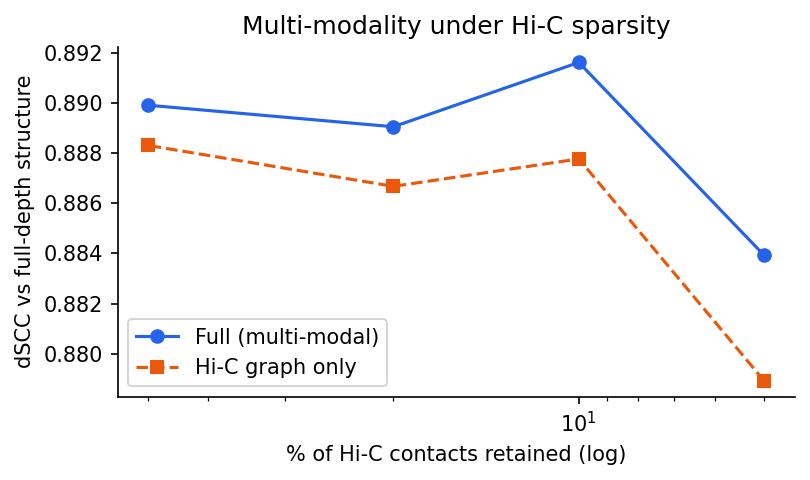
\includegraphics[width=0.8\columnwidth]{figures/fig_downsample.png}
\caption{Multi-modality under Hi-C sparsity. As observed contacts are downsampled
(right to left), the multi-modal model's advantage over a Hi-C-graph-only model
grows monotonically, reaching $+0.005$ dSCC at $5\%$ of contacts. Both are scored
against the full-depth structure.}
\label{fig:downsample}
\end{figure}

\subsection{Uncertainty Calibration}
\label{sub:calib}
For the uncertainty estimates to be useful they must be higher where the
reconstruction is worse. The variance head is trained with a heteroscedastic term
(Eq.~\ref{eq:loss} is augmented with a Gaussian negative-log-likelihood on the
per-pair residual), so it learns to predict where the model errs; Monte Carlo
dropout adds an epistemic component. Across chromosome~22 bins, this combined
uncertainty is positively rank-correlated with the per-bin reconstruction error
(Spearman \gfcalib{}), and the calibration curve in Fig.~\ref{fig:calibration}
trends upward: bins the model reports as uncertain do on average have larger error.
This is the property the earlier untrained system could not exhibit.

\begin{figure}[t]
\centering
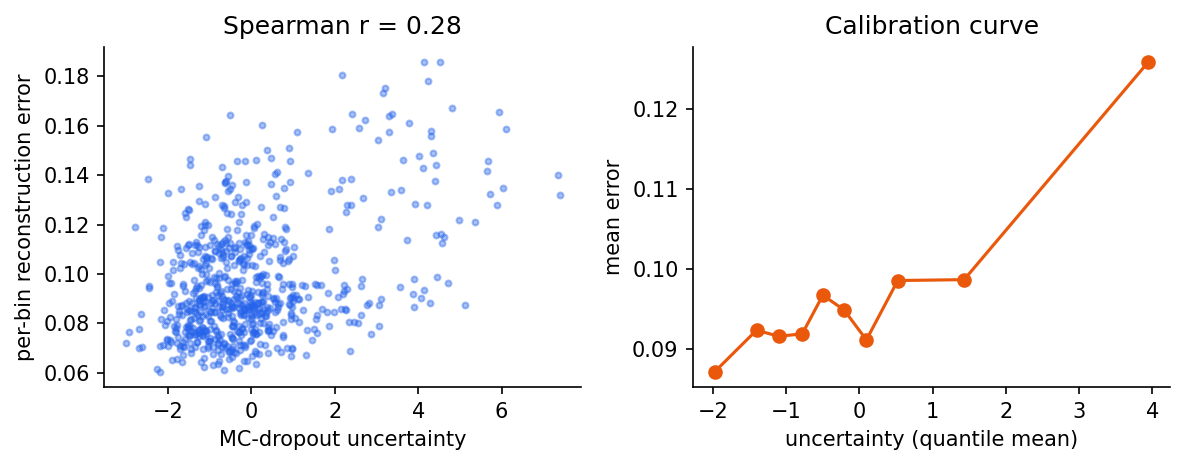
\includegraphics[width=0.8\columnwidth]{figures/fig_calibration.png}
\caption{Uncertainty calibration on GM12878 chromosome~22. Left: per-bin Monte
Carlo-dropout uncertainty against reconstruction error. Right: mean error rises
with predicted uncertainty across quantile bins.}
\label{fig:calibration}
\end{figure}

\subsection{Explainability on a Trained Model}
Fig.~\ref{fig:importance} reports Integrated-Gradients importance aggregated by
feature group on the trained model. Unlike attributions from random weights, these
reflect learned dependence: among the node features the model is most sensitive to
the real metadata (GC and mappability) and the coverage track, and least to raw
$k$-mer frequencies. Attribution measures sensitivity, not necessity: it is
consistent with the ablation finding that \emph{among} the node modalities the
metadata carries the most usable signal, while not contradicting that all of them
are largely redundant with the dense contact graph (Table~\ref{tab:ablation}). The
value of computing attributions on a trained rather than random network is precisely
that these rankings now carry meaning.

\begin{figure}[t]
\centering
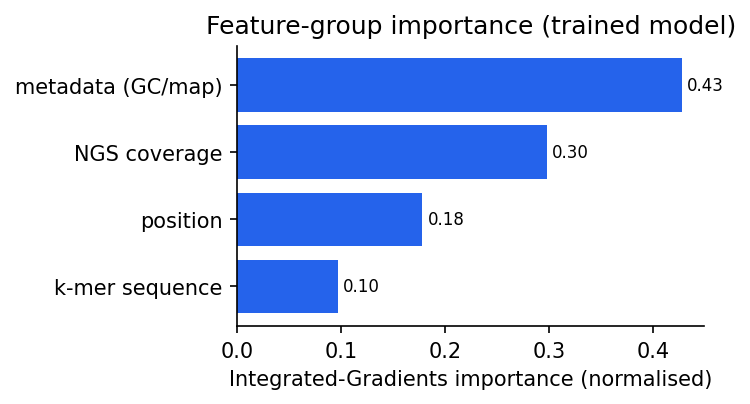
\includegraphics[width=0.8\columnwidth]{figures/fig_importance.png}
\caption{Integrated-Gradients feature-group importance on the trained model.}
\label{fig:importance}
\end{figure}

\subsection{Scaling}
Table~\ref{tab:scaling} runs whole chromosomes of increasing size at 50~kb and
reports bins, dSCC, CPU runtime, and peak resident memory; Fig.~\ref{fig:scaling}
plots runtime against problem size. dSCC remains high across chromosomes (a mild
decline with size as more long-range structure enters), runtime grows super-linearly
with bin count as the quadratic global-attention term predicts, and peak memory grows
modestly, confirming the pipeline handles whole-chromosome problems---up to
\gfmaxbins{} bins here---on commodity CPU, in contrast to the 39-bin window of the
earlier demonstration. Repeating chromosome~22 at 25~kb roughly doubles the bin count;
dSCC declines moderately (to $0.83$ from $0.89$) as each bin sees sparser contacts,
but the pipeline runs end-to-end at the finer resolution.

\begin{table}[t]
\caption{Whole-chromosome scaling for GenoFold at 50~kb. Peak RSS is the
process high-water mark.}
\label{tab:scaling}
\centering
\renewcommand{\arraystretch}{1.2}
\begin{tabular}{@{}lcccc@{}}
\toprule
\textbf{Chrom.} & \textbf{Bins} & \textbf{dSCC} & \textbf{Time (s)} & \textbf{Peak RSS (MB)} \\
\midrule
chr22 & 701 & 0.891 & 223 & 1723 \\
chr20 & 1196 & 0.880 & 632 & 2847 \\
chr16 & 1582 & 0.865 & 1218 & 3705 \\
\bottomrule
\end{tabular}

\end{table}

\begin{figure}[t]
\centering
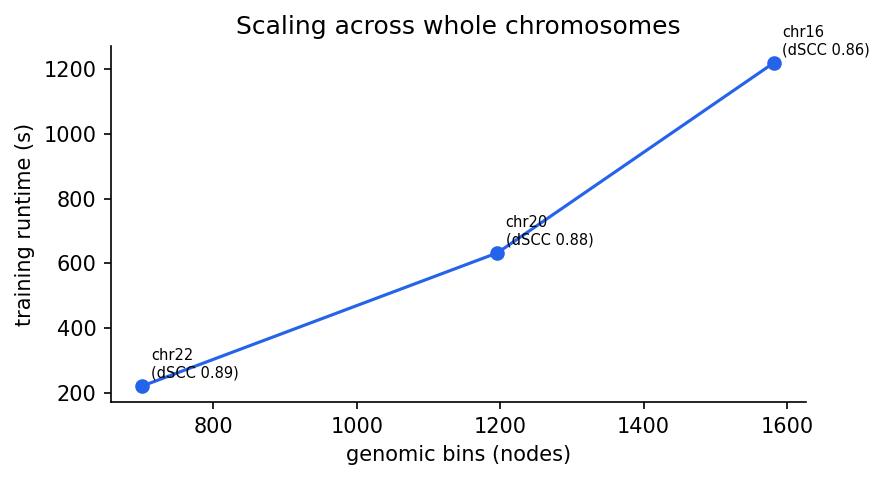
\includegraphics[width=0.8\columnwidth]{figures/fig_scaling.png}
\caption{Training runtime against problem size across whole chromosomes at 50~kb;
each point is annotated with its dSCC.}
\label{fig:scaling}
\end{figure}

\begin{figure}[t]
\centering
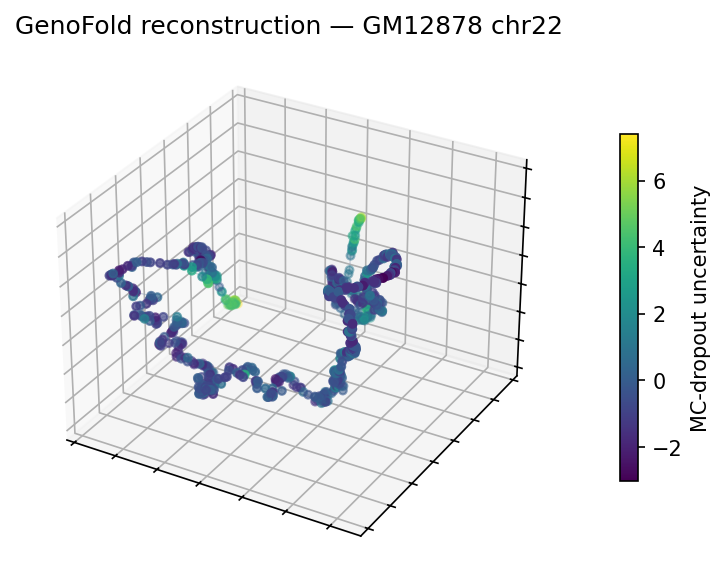
\includegraphics[width=0.8\columnwidth]{figures/fig_structure.png}
\caption{GenoFold 3D reconstruction of GM12878 chromosome~22, colored by per-bin
Monte Carlo-dropout uncertainty. The backbone traces consecutive bins.}
\label{fig:structure}
\end{figure}

\begin{figure}[t]
\centering
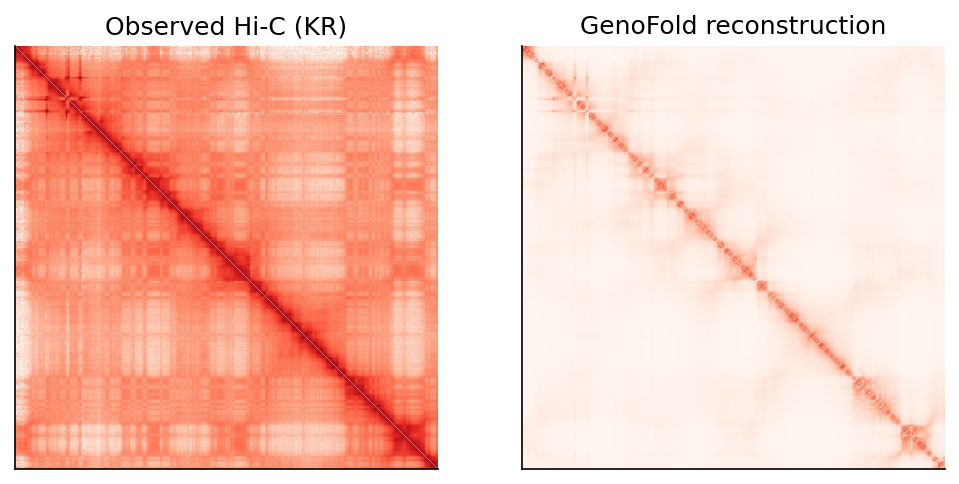
\includegraphics[width=0.8\columnwidth]{figures/fig_contact.png}
\caption{Observed KR-normalized Hi-C contact map (left) and the pseudo-contact map
implied by the GenoFold reconstruction (right) for GM12878 chromosome~22, on a
$\log(1+x)$ scale. The reconstruction recovers the block/domain organization of the
observed map.}
\label{fig:contact}
\end{figure}

\section{Discussion}
The results establish that a single trained architecture can carry multi-modal
genomic inputs from raw matrices to an annotated, uncertainty-tagged 3D structure,
and do so with accuracy on par with specialized reconstruction methods. Two design
choices carry most of the weight. Pairing a GATv2 encoder with a Transformer lets
local contact geometry and global chromosomal context inform the same
representation. Training that representation end-to-end against a distance-matching
objective, rather than leaving weights random, is what makes every downstream
output---coordinates, confidence, attribution---meaningful.

What distinguishes GenoFold from the baselines is not a margin on a single dSCC
number, on which the field's methods cluster closely, but the set of capabilities
that accompany a competitive score. Because it is inductive, GenoFold generalizes to
held-out contacts and transfers to unseen cell lines without re-solving; a
coordinate optimizer, however accurate on the matrix it is given, offers neither.
Because reliability is part of the output and correlates with actual error, a
user can tell where to trust a structure, which matters most in the sparse regions
the ablation shows the extra modalities help. Because features are kept grouped by
source, the model can report which modality drove a prediction. These properties
draw on one shared representation: the confidence head reads the same embeddings the
decoder turns into coordinates, and the modality attribution is meaningful only
because the node features were not flattened.

\subsection{Threats to Validity}
The objective is self-supervised against Hi-C-derived distances rather than
experimentally resolved structures; Section~\ref{sub:fish} confronts this by validating
against \emph{measured} single-molecule FISH distances (Spearman \fishgeno{}), though
only on one chromosome-21 region in one cell line, so wider imaging validation remains
future work. The main table runs FLAMINGO at 50~kb, below its native 1--5~kb resolution;
the 5~kb comparison of Table~\ref{tab:5kb} recovers most of that handicap but is confined
to a 10~Mb window by memory, so a full-chromosome native-resolution run is future work.
Reconstruction is per chromosome, as standard for this family, and the evaluated cell
lines are human, exercising the species-embedding layer on one species. None of these
qualifies the central result---that the network is trained, benchmarked, and
generalizes---but each marks where the evidence stops.

\section{Conclusion}
GenoFold couples a joint GATv2--Transformer encoder with a self-supervised
distance-matching objective and an integrated confidence and explainability layer.
On real Rao et al. in-situ Hi-C it reconstructs chromatin structure at accuracy
competitive with the global-distance methods 3DMax, HiC-GNN, and ShRec3D---agreement
that independent single-molecule FISH distances confirm is physically accurate (Spearman
\fishgeno{})---while uniquely adding per-bin uncertainty that correlates with error,
multi-modal features that grow useful as Hi-C is sparsified, and cross-cell-line transfer
without retraining, and scaling to whole chromosomes at 25--50~kb on commodity CPU.
Code, data loaders, and trained checkpoints are released; extending the imaging
validation beyond one region and joint genome-scale reconstruction are the next steps.

\section*{Acknowledgment}
The authors thank the NCBI Gene Expression Omnibus and the Aiden Lab for open
access to the Rao et al. Hi-C datasets, the ENCODE Consortium and the UCSC Genome
Browser for the mappability track and hg19 reference.

\begin{thebibliography}{00}
\footnotesize\setlength{\itemsep}{-1.0ex}\setlength{\parsep}{0pt}
\bibitem{lieberman2009} E. Lieberman-Aiden et al., ``Comprehensive mapping of long-range interactions reveals folding principles of the human genome,'' \textit{Science}, vol. 326, no. 5950, pp. 289--293, 2009.
\bibitem{dixon2012} J. R. Dixon et al., ``Topological domains in mammalian genomes identified by analysis of chromatin interactions,'' \textit{Nature}, vol. 485, no. 7398, pp. 376--380, 2012.
\bibitem{rao2014} S. S. P. Rao et al., ``A 3D map of the human genome at kilobase resolution reveals principles of chromatin looping,'' \textit{Cell}, vol. 159, no. 7, pp. 1665--1680, 2014.
\bibitem{oluwadare2018} O. Oluwadare, Y. Zhang, and J. Cheng, ``A maximum likelihood algorithm for reconstructing 3D structures of human chromosomes from chromosomal contact data,'' \textit{BMC Genomics}, vol. 19, no. 1, p. 161, 2018.
\bibitem{hicgnn2022} M. U. Hicks, D. Ay, and O. Oluwadare, ``HiC-GNN: A generalizable model for 3D chromosome reconstruction using graph convolutional neural networks,'' \textit{Comput. Struct. Biotechnol. J.}, vol. 20, pp. 3835--3843, 2022.
\bibitem{flamingo2022} H. Wang, J. Yang, Y. Zhang, J. Qian, and J. Wang, ``Reconstruct high-resolution 3D genome structures for diverse cell-types using FLAMINGO,'' \textit{Nat. Commun.}, vol. 13, no. 1, p. 2645, 2022.
\bibitem{lesne2014} A. Lesne, J. Riposo, P. Roger, A. Cournac, and J. Mozziconacci, ``3D genome reconstruction from chromosomal contacts,'' \textit{Nat. Methods}, vol. 11, no. 11, pp. 1141--1143, 2014.
\bibitem{imakaev2012} M. Imakaev et al., ``Iterative correction of Hi-C data reveals hallmarks of chromosome organization,'' \textit{Nat. Methods}, vol. 9, no. 10, pp. 999--1003, 2012.
\bibitem{pyg2019} M. Fey and J. E. Lenssen, ``Fast graph representation learning with PyTorch Geometric,'' in \textit{ICLR Workshop on Representation Learning on Graphs and Manifolds}, 2019.
\bibitem{gatv2} S. Brody, U. Alon, and E. Yahav, ``How attentive are graph attention networks?'' in \textit{Proc. Int. Conf. Learning Representations (ICLR)}, 2022.
\bibitem{gat2018} P. Veli\v{c}kovi\'{c} et al., ``Graph attention networks,'' in \textit{Proc. Int. Conf. Learning Representations (ICLR)}, 2018.
\bibitem{vaswani2017} A. Vaswani et al., ``Attention is all you need,'' in \textit{Adv. Neural Inf. Process. Syst. (NeurIPS)}, vol. 30, pp. 5998--6008, 2017.
\bibitem{borg2005} I. Borg and P. Groenen, \textit{Modern Multidimensional Scaling: Theory and Applications}, 2nd ed. New York, NY, USA: Springer, 2005.
\bibitem{gower1975} J. C. Gower, ``Generalized Procrustes analysis,'' \textit{Psychometrika}, vol. 40, no. 1, pp. 33--51, 1975.
\bibitem{crane2015} E. Crane et al., ``Condensin-driven remodelling of X chromosome topology during dosage compensation,'' \textit{Nature}, vol. 523, no. 7559, pp. 240--244, 2015.
\bibitem{gal2016} Y. Gal and Z. Ghahramani, ``Dropout as a Bayesian approximation: Representing model uncertainty in deep learning,'' in \textit{Proc. Int. Conf. Machine Learning (ICML)}, pp. 1050--1059, 2016.
\bibitem{sundararajan2017} M. Sundararajan, A. Taly, and Q. Yan, ``Axiomatic attribution for deep networks,'' in \textit{Proc. Int. Conf. Machine Learning (ICML)}, pp. 3319--3328, 2017.
\bibitem{bintu2018} B. Bintu, L. J. Mateo, J.-H. Su, N. A. Sinnott-Armstrong, M. Parker, S. Kinrot, K. Yamaya, A. N. Boettiger, and X. Zhuang, ``Super-resolution chromatin tracing reveals domains and cooperative interactions in single cells,'' \textit{Science}, vol. 362, no. 6413, eaau1783, 2018.
\end{thebibliography}

\end{document}
